\documentclass[a4paper]{article}
\usepackage[UTF8]{ctex}
\usepackage{geometry}
\usepackage{graphicx}
\usepackage{url}
\usepackage{multirow}
\usepackage{array}
\usepackage{booktabs}
\usepackage{url}
\usepackage{enumitem}
\usepackage{graphicx}
\usepackage{float}
\usepackage{amssymb}
\usepackage{amsmath}
\usepackage{subfig}
\usepackage{longtable}
\usepackage{pifont}
\usepackage{color}

\allowdisplaybreaks

\geometry{a4paper, scale=0.78}

\usepackage{tikz}
\newcommand*{\circled}[1]{\lower.7ex\hbox{\tikz\draw (0pt, 0pt)%
    circle (.5em) node {\makebox[1em][c]{\small #1}};}}

% \begin{figure}[H]
%     \centering
%     \includegraphics[width=.55\textwidth]{E.png}
%     \caption{矩阵与列向量的乘法}
%     \label{fig:my_label_1}
% \end{figure}

% \left\{
% \begin{array}{ll}
%       x+2x+z=2 & \\
%       3x+8y+z=12 & \\
%       4y+z=2
% \end{array}
% \right.

% \begin{enumerate}[itemindent = 1em, itemsep = 0.4pt, parsep=0.5pt, topsep = 0.5pt]

% \end{enumerate}

%\stackrel{a}{\longrightarrow}

%\underbrace{}_{} %下括号

%\triangleq %等式上加三角形

%\tableofcontents %目录,并且目录页不记录页码
% \tableofcontents
% \newpage
% \setcounter{page}{1} %new page
% \clearpage

\title{Reinforcement Learning Dynamic Programming}
\author{Chen Gong}
\date{20 July 2020}
\begin{document}
%\pagestyle{empty}

\maketitle
\tableofcontents
\newpage
\setcounter{page}{1} %new page
%\pagestyle{fancy}
\section{Background}
本小节介绍动态规划的主要目的是通过动态规划来求解得到最优策略$\pi^\ast$,从而使得价值函数最高。当然上一小节中我们已经证明了,最优策略对应的就是最优价值函数。求解方法基本上就是从两个角度出发,1. 策略迭代,2. 价值迭代。

策略迭代可以分成两步,策略评估和策略改进。策略改进为即固定价值函数,并且找到在该价值函数下的最优策略,也就是估计策略评估得出的$V^\pi(s)$,寻找一个新的策略$\pi'$使得$V^{\pi'}(s) > V^{\pi}(s)$。另一步称作策略估计(policy evaluation),即固定策略,找出该策略下的价值函数,也就是根据$\pi$,对$\forall s$,求解$Q^\pi(s,a),V^\pi(s,a)$。

\section{策略评估,解析解}
\subsection{策略评估解析解推导}
所谓策略评估,就是已知MDP模型,即为$P(s',r|s,a)$都知道的情况下。给定$\pi$求解$V^\pi(s)\ (\forall s \in \mathcal{S})$。我们把$V^\pi(s)$当成一个向量,记为,
\begin{equation}
    V^\pi(s) = 
    \begin{bmatrix}
         V^\pi(s_1) \\
         V^\pi(s_2) \\
         \vdots \\
         V^\pi(s_{|s|})
    \end{bmatrix}_{|s|\times 1}
\end{equation}
而贝尔曼方程可以写为如下形式,准确的说是一个方程组,因为每一个状态都对应一个方程组。
\begin{equation}\begin{aligned}
V^{\pi}(s) &=\mathbb{E}_{\pi}\left[G_{t} \mid S_{t}=s\right] \\
&=\mathbb{E}_{\pi}\left[R_{t+1}+\gamma V^{\pi}\left(s_{t+1}\right) \mid s_{t}=s\right] \\
&=\sum_{a} \pi(a \mid s) \cdot \sum_{s^{\prime}, r} p\left(s' , r \mid s,a\right)\left[r+\gamma V^{\pi}\left(s^{\prime}\right)\right]
\end{aligned}\end{equation}
很显然,根据上式,我们可以看到$V^{\pi}(s)$和$V^{\pi}\left(s^{\prime}\right)$之间是线性关系。由于是线性关系那就好办了,我们可以用矩阵的形式来表示到$V^{\pi}(s)$和$V^{\pi}\left(s^{\prime}\right)$之间的关系。其中一共有$|s|$个状态,那么化简方法也很简单只要把(2)式拆开一步步化简就行了,具体过程如下所示,
\begin{equation}
    V^{\pi}(s) = \underbrace{\sum_{a} \pi(a \mid s) \cdot \sum_{s^{\prime}, r} p\left(s' , r \mid s,a\right) r}_{\circled{1}} + \underbrace{\gamma \sum_{a} \pi(a \mid s) \cdot \sum_{s^{\prime}, r} p\left(s' , r \mid s,a\right) V^{\pi}\left(s^{\prime}\right)}_{\circled{2}}
\end{equation}
其中第一项,可以将$\sum_{s^{\prime}, r} p\left(s' , r \mid s,a\right) r$中的$s$积分掉,那么可以化简为$\sum_{a} \pi(a \mid s) \cdot \sum_{ r} p\left( r \mid s,a\right) r$。很显然,$\sum_{ r} p\left( r \mid s,a\right) r$这一项就是一个期望,那么我们可以将当前时刻的奖励函数$r(s,a)$定义为$\sum_{ r} r p\left( r \mid s,a\right) $。将其改写为积分形式可以得到,
\begin{equation}
   r(s,a) \triangleq \mathbb{E}_\pi [R_{t+1}|s_t=s,a_t=a]
\end{equation}
那么,\circled{1}可以表达为$\sum_{a} \pi(a \mid s) \cdot r(s,a)$。由于对$a$进行积分,其中$\pi$是一个关于$a$的概率分布。那么所有和$a$的项都可以去掉,得到最终的化简结果为,
\begin{equation}
    \circled{1} = r_\pi(s)
\end{equation}
那么,根据推导得出的关于\circled{1}的结果可以用一个矩阵来表示,
\begin{equation}
    r_\pi = 
    \begin{bmatrix}
        r_\pi (s_1) \\
        r_\pi (s_2) \\
        \vdots \\
        r_\pi (s_{|s|}) \\
    \end{bmatrix}_{|s| \times 1}
\end{equation}
同理,针对第二项,可以做如下的推导,
\begin{equation}
    \begin{aligned}
        \circled{2} = & \gamma \sum_{a} \pi(a \mid s) \cdot \sum_{s^{\prime}, r} p\left(s' , r \mid s,a\right) V^{\pi}\left(s^{\prime}\right) \\
        = & \gamma \sum_{a} \pi(a \mid s) \cdot \sum_{s^{\prime}} p\left(s' \mid s,a\right) V^{\pi}\left(s^{\prime}\right) \\
        = & \gamma \sum_{a} \sum_{s^{\prime}} \pi(a \mid s) \cdot  p\left(s' \mid s,a\right) V^{\pi}\left(s^{\prime}\right) \\
    \end{aligned}
\end{equation}
其中令$P^\pi(s,s') = \sum_a \pi(a \mid s) \cdot  p\left(s' \mid s,a\right)$。那么有,
\begin{equation}
    \circled{2} = \gamma P^\pi(s,s') V^{\pi}\left(s^{\prime}\right)
\end{equation}
其中$P^\pi(s,s')$是关于$s,s'$之间的转移概率,所以是维度为$|s|\times |s|$的矩阵,记为$P^\pi \triangleq \left[ P^\pi(s,s') \right]_{|s| \times |s|}$。显然,公式(3)被我们化简为,
\begin{equation}
    V^\pi(s) = r_\pi(s) + \gamma P^\pi(s,s') V^{\pi}\left(s^{\prime}\right)
\end{equation}
将$s_i \triangleq s$,$s_j \triangleq s'$,我们可以得到如下化简。
\begin{equation}
    V^\pi(s_i) = r_\pi(s_i) + \gamma \sum_{j=1}^{|s|} P^\pi(s_i,s_j) V^{\pi}\left(s_j\right)
\end{equation}
我们可以简写为,
\begin{equation}
\begin{aligned}
    V^\pi = & r_\pi + \gamma P^\pi V^\pi \\
    (I-\gamma P^\pi)V^\pi = & r_\pi \\
    V^\pi = & (I-\gamma P^\pi)^{-1}r_\pi \\
\end{aligned}
\end{equation}

\subsection{策略评估解析解小结}
策略评估的目的是在给定$\pi$的情况下,求解$V^\pi$。根据贝尔曼方程,
\begin{equation}\begin{aligned}
V^{\pi}(s)
&=\sum_{a} \pi(a \mid s) \cdot \sum_{s^{\prime}, r} p\left(s' , r \mid s,a\right)\left[r+\gamma V^{\pi}\left(s^{\prime}\right)\right]
\end{aligned}\end{equation}
可以推导得到,$V^\pi$的解析解为,
\begin{equation}
    V^\pi = (I-\gamma P^\pi)^{-1}r_\pi
\end{equation}


那么经过上述的推导,我们计算出来$V^\pi$的解析解,它是一个维度为$|s|\times 1$的矩阵。但是,问题就来了,其求解难度太大了,计算复杂度为$\mathcal{O}(|s|^3)$,而且还涉及到矩阵的求逆,当状态空间足够多的时候,计算难度非常大。

\section{策略评估,迭代解}
本章针对上一小节求解$V^\pi(s)$解析解过于复杂的问题,讲解另一种新的解决思路,即为迭代策略估计。第一种方法实际上就是解析解,而第二种方法用迭代的方法得到的是数值解。

具体思路就是构造一个数列$\{V^k\}_{k=1}^\infty$,让其可以收敛到$V^\pi(s)$。其中$V^k$代指的都是函数向量,举例说明,
\begin{equation}
    V^1=
    \begin{bmatrix}
    V^1(s_1) \\
    V^1(s_2) \\
    \vdots \\
    V^1(s_{|s|}) \\
    \end{bmatrix}
\end{equation}
因为需要迭代,所以下一步需要知道$V^k$与$V^{k+1}$之间的关系。我们估计贝尔曼方程动态的构建$V^k$与$V^{k+1}$之间的关系。根据贝尔曼方程,我们可以类似的写出其迭代关系为,
\begin{equation}
   V^{k+1}(s) =\sum_{a} \pi(a \mid s) \cdot \sum_{s^{\prime}, r} p\left(s' , r \mid s,a\right)\left[r+\gamma V^{k}\left(s^{\prime}\right)\right] 
\end{equation}
其中,$v^1$是一个随机的初始函数向量。而在上一节“马尔可夫决策过程”中,我们已经证明过使用贝尔曼方程迭代,根据压缩映射定理,可以收敛到唯一的最优解了。

其实,我们可以看到。我们可以依赖的只有贝尔曼方程,通过对贝尔曼方程的迭代来计算价值函数。其实整体思路还是比较简单。

\section{策略改进定理}
策略评估完成之后,下一步当然就是策略改进了。什么是策略改进呢?也就是给你一个$\pi$,你将其转换为$\pi'$。使得$\pi'>\pi$,即为$\forall s\in \mathcal{S},V^{\pi'}(s) > V^{\pi}(s)$。而马上又遇到新的问题了,要求$V^{\pi'}(s),V^{\pi}(s)$,我们需要对两个策略来求解价值函数。

那么针对这个问题,提出了策略改进定理,我们只需要求一个$V^{\pi}(s)$就可以了,这个定理是什么呢?\textbf{给定$\pi,\pi'$,如果对于任意状态$s$,$Q^\pi(s,\pi'(s))\geq V^\pi(s)$,那么则有$\forall s\in \mathcal{S}, V^{\pi'}(s) \geq V^\pi(s)$。}通过这个定理,很显然我们看到只需要求解关于$\pi$的价值函数即可,求解出$Q^\pi(s,a)$,也就相当于求解出了$V^\pi(s)$。那么,为什么呢?下面进行证明,

\subsection{策略改进定理的证明}
我们的目的是证明,$\forall s \in \mathcal{S}$,有$V^\pi(s) \leq Q^\pi(s,\pi'(s))$。那么求解思路就是,想办法使用$Q^\pi(s,\pi'(s))$构建一个放缩关系,使得$V^\pi(s) \leq V^{\pi'}(s)$。其中$V^\pi(s)$中所有的$a$都是由$\pi$控制的,而$V^{\pi'}(s)$中所有的$a$都是由$\pi'$控制的。这里$Q^\pi(s,\pi'(s))$就比较有意思了,好像正好是介于两者之间。首先简单惠顾一下$Q(s,a)$的定义,
\begin{equation}\begin{aligned}
Q^{\pi}(s, a) &=\sum_{s^{\prime}, r} p\left(s^{\prime}, r \mid s, a\right)\left[r+\gamma V^{\pi}\left(s^{\prime}\right)\right] \\
&=\mathbb{E}_{\pi}\left[R_{t+1}+\gamma V^{
\pi}\left(s_{t+1}\right) \mid s_{t}=s,a_t =a\right]
\end{aligned}\end{equation}
注意这里,提到$R_{t+1}$实际上和$\pi$是没有关系的,为什么呢?$R_{t+1}$表示的是当前状态$s$执行动作$a$获得的平均回报,显然$s,a$之间是由$\pi$给出的映射,而在$Q^\pi(s,a)$中$s,a$并没有直接关系,并不是通过$\pi:s\to a$得到的。所以,产生的$R_{t+1}$当然也是和$\pi$没有关系。如果是用$Q^\pi(s,a) = \mathbb{E}_\pi[G_t|s_t=s,a_t=a]$,当然在这里使用$\pi$下标没有关系,如果是拆开的话,那么更加严格的写法为如下所示。\textbf{$Q^\pi(s,a)$大致可以理解为,从当前状态选择$s_t$其实是随意的,而从$s_{t+1}$状态之后动作$a$的选择都是由$\pi$来确定的。}
\begin{equation}
    Q^\pi(s,a) = \mathbb{E}\left[R_{t+1}+\gamma V^{
\pi}\left(s_{t+1}\right) \mid s_{t}=s,a_t =a\right]
\end{equation}
接下来开始证明推导过程,
\begin{equation}
    \begin{aligned}
        V^\pi(s) \leq & Q^\pi(s,\pi'(s)) \\
        = & \mathbb{E}\left[R_{t+1}+\gamma V^{
        \pi}\left(s_{t+1}\right) \mid s_{t}=s,a_t =\pi'(s)\right] \\
        = & \mathbb{E}_{\pi'}\left[R_{t+1}+\gamma V^{
        \pi}\left(s_{t+1}\right) \mid s_{t}=s\right] \\
    \end{aligned}
\end{equation}
这里是为什么呢?因为现在已经很明确了$\pi':s\to a$,所以$R_{t+1}$的得到完全是由$\pi'$控制的。所以,我们可以改写为公式(18)中的形式。此公式表示的为$t$时刻的动作由$\pi'$来确定,而之后的$t+n$时刻的状态还是由$\pi$来确定。那么,接着公式(18)继续进行推导可以得到,
\begin{equation}
    \begin{aligned}
        V^\pi(s) \leq & Q^\pi(s,\pi'(s)) \\
        = & \mathbb{E}\left[R_{t+1}+\gamma V^{
        \pi}\left(s_{t+1}\right) \mid s_{t}=s,a_t =\pi'(s)\right] \\
        = & \mathbb{E}_{\pi'}\left[R_{t+1}+\gamma V^{
        \pi}\left(s_{t+1}\right) \mid s_{t}=s\right] \\
        \leq & \mathbb{E}_{\pi'}\left[R_{t+1}+\gamma Q^\pi(s_{t+1},\pi'(s_{t+1})) \mid s_{t}=s\right] \\
        = & \mathbb{E}_{\pi'}\left[R_{t+1}+\gamma \mathbb{E}_{\pi'}\left[ R_{t+2} + \gamma V^\pi(s_{t+1}) \mid s_{t+1} \right] \mid s_{t}=s\right] \\
        = & \mathbb{E}_{\pi'}\left[R_{t+1}+\gamma \mathbb{E}_{\pi'}\left[ R_{t+2}|s_{t+1} \right] + \gamma^2 \mathbb{E}_{\pi'}\left[ V^\pi(s_{t+1}) \mid s_{t+1} \right] \mid s_{t}=s\right] \\
        = & \mathbb{E}_{\pi'}\left[R_{t+1}+\gamma R_{t+2} + \gamma^2  V^\pi(s_{t+1}) \mid s_{t}=s\right] \\
        = & \cdots \\
        \leq & \mathbb{E}_{\pi'}[\underbrace{R_{t+1}+\gamma R_{t+2} + \gamma^2 R_{t+3} + \cdots + \cdots}_{G_t} \mid s_{t}=s] \\
        = & V^{\pi'}(s)
        \end{aligned}
\end{equation}

\subsection{贪心策略}
上一小节中推导了策略改进定理,这是一种可以快速比较两个策略谁优谁劣的方法。这小节,描述的是,如何利用策略改进定理,来优化当前策略。

首先,利用policy evaluation根据$\pi\to Q^\pi(s,a)$。然后根据$Q^\pi(s,a)$改进得到$\pi'$。采用的改进方法是Greedy Policy贪心策略。用公式化的语言描述就是,$\forall s\in \mathcal{S},\pi'(s) = \underset{a}{\arg\max} Q^\pi(s,a)$。对于每个状态$s$,我们都选取使得$Q^\pi(s,a)$最大的函数,这样就可以得到一个$\pi'$。下一步就要结合策略改进定理,证明得到的$\pi'(s)$优于$\pi(s)$。

根据“马尔可夫决策过程”那一章的知识可得,$\forall s \in \mathcal{S},\forall V^\pi(s) \leq \max_a Q^\pi(s,a) = Q^\pi(s,\pi'(s)$。根据策略改进定理,我们就直接得证了,确实$\forall s\in \mathcal{S},V^{\pi'}(s) \geq V^\pi(s)$。

就这样反复迭代下去,如果在某一时刻$V^{\pi'}(s) = V^\pi(s)$,则说明算法已经收敛,那么很显然有$\pi = \pi' = \pi^\ast$。因为压缩映射定理表明,可以收到到唯一的最优解。这里也可以用其他的方法简单的证明一下,

证明,我们的条件有$V^{\pi^{\prime}}=V^{\pi} \Rightarrow Q^{\pi^{\prime}}=Q^{\pi}$。

$\forall s\in \mathcal{S}$有,
\begin{equation}
\begin{aligned}
    V^{\pi'}(s) = & \sum_a \pi'(a|s) Q^{\pi'}(s,a)\\
    = & \sum_a \pi'(a|s) Q^{\pi}(s,a) \\
    = & Q^{\pi}(s,\pi'(a|s)) \\
    = & \max_a Q^{\pi}(s,a) \\
    = & \max_a \sum_{s',r} P(s',r|s,a)[r + \gamma V^\pi(s')] \\
    = & \max_a \sum_{s',r} P(s',r|s,a)[r + \gamma V^{\pi'}(s')]
\end{aligned}
\end{equation}
整理可得,
\begin{equation}
    V^{\pi'}(s) = \max_a \sum_{s',r} P(s',r|s,a)[r + \gamma V^{\pi'}(s')]
\end{equation}
实际上这就是Bellman Optimality Equation,同样可以写为,
\begin{equation}
    V^{\ast}(s) = \max_a \sum_{s',r} P(s',r|s,a)[r + \gamma V^{\ast}(s')]
\end{equation}
所以,可以得到$\pi = \pi' = \pi^\ast$。基本上到这里策略迭代的基本内容就结束了。

\section{价值迭代}
\subsection{策略迭代$\to$价值迭代}
上一小节中,我们详细的介绍了策略迭代。策略迭代一般可以分成两步,1. 策略评估,由$\pi \to V^\pi(s)$,采用的是迭代的方法。2. 策略改进,使用的是greedy($s$)。而策略迭代和策略评估合在一起执行一次,称之为策略迭代的一次迭代。

但是这样做会有一个麻烦,就是迭代中套迭代。首先外层要迭代求解$\pi^\ast$,而且每一次求解的过程中还要迭代的求$V^\pi$,模型过程一般为$\pi_1 \to V^{\pi_1} \to \pi_2 \to V^{\pi_2} \to \cdots \to V^{\pi_{\ast}} $。所以计算就很麻烦。于是,有了截断策略评估的方法,\textbf{其中心思想是对于每个$\pi$,并不精准计算$V^\pi$,而是计算$V^\pi$的近似值。}具体的做法是,计算$V$函数本就是用到了迭代的方法,可能原本计算精准值需要迭代100次,现在只迭代80次,或者最极端的情况只迭代一次,计算一个模糊的价值函数。

极端情况就是策略评估中只进行一步迭代,然后进行策略改进,这时得到的就是贝尔曼最优方程,
\begin{equation}
    V^{k+1}(s) = \max_a \sum_{s',r} P(s',r|s,a)[r + \gamma V^{k}(s')]
\end{equation}
下面将进一步详细的描述,我相信很多同学看到这里会有点懵逼。首先对于策略评估的一次迭代就是,
\begin{equation}
    Q^{k+1}(s,a) = \sum_{s',r} P(s',r\mid s,a)[r+\gamma V^{k}(s')]
\end{equation}
这里很显然是每一次策略迭代中策略评估只进行一次迭代。大家注意到根据贝尔曼方程应该是$V^{k+1}(s) = \sum_{s',r} P(s',r\mid s,a)[r+\gamma V^{k}(s')]$。而这里的公式里为什么是$Q^{k+1}(s,a)$呢?我们看看如下图中的示例,
\begin{figure}[H]
    \centering
    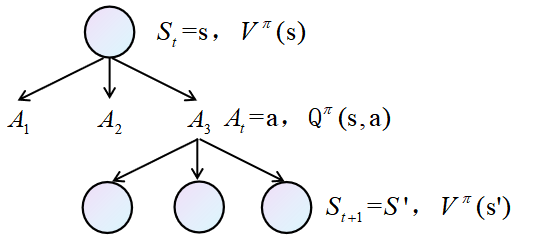
\includegraphics[width=.55\textwidth]{微信图片_20200726193005.png}
    \caption{马尔可夫决策过程示例}
    \label{fig:my_label_1}
\end{figure}
与其说我们进行了一步迭代,不如说一步都没有,只有半步。实际上只更新了$Q^\pi(s,a)$,而没有走下一步$Q^\pi(s,a)\to V^\pi(s')$。而通过greedy方法来得到$V^\pi(s')$。

所以,首先计算的是公式(24)。然后通过,
\begin{equation}
    \begin{aligned}
        & \max_a Q^{k+1}(s,a) = \max_a \sum_{s',r} P(s',r\mid s,a)[r+\gamma V^{k}(s')] \\
        & V^{\pi'}(s) = \max_a Q^{k+1}(s,a) = \max_a \sum_{s',r} P(s',r\mid s,a)[r+\gamma V^{k}(s')] \\
    \end{aligned}
\end{equation}
所以,这样的迭代中,我们不在需要通过反复迭代来求解$V^\pi(s)$。整体的求解轨迹为:$V^1(s)\to V^2(s)\to V^3(s)\to \cdots\to V^\ast(s)$。这就是价值迭代,\textbf{所以,从策略迭代的角度出发来看,价值迭代就是极端情况下的策略迭代。}

\subsection{价值迭代$\to$就地策略迭代}
我觉得从价值函数角度来理解,没有这么的绕。我们可以直接将其理解为对于价值函数的迭代,通过求解轨迹$V^1(s)\to V^2(s)\to V^3(s)\to \cdots\to V^\ast(s)$来得出最优价值函数。

而在策略迭代中,我们使用的是$V^{\pi'}(s) = \max_a \sum_{s',r} P(s',r\mid s,a)[r+\gamma V^{k}(s')]$。那么针对状态集合$\mathcal{S}$中的每一个状态都要更新,需要遍历整个状态空间,
\begin{equation}
    \begin{aligned}
    & V^{k+1}(s_1) = \cdots \\
    & V^{k+1}(s_2) = \cdots \\
    & \vdots \\
    & V^{k+1}(s_{|s|}) = \cdots \\
    \end{aligned}
\end{equation}
但是,大家发现这样更新同样麻烦。于是,科学家们想了一个办法,在第$k$次更新中,不对状态集合$\mathcal{S}$中的每一个状态都更新,而只随机选取其中的某一个状态的$V^k{s_n}$进行更新,其他状态保持不变。这就是就地策略迭代,也是一种特殊的异步策略迭代方法。大家其实都发现了,我们都在想办法来简化策略评估的计算来减少整体的计算量。因为,策略评估可优化的空间最大。
\begin{figure}[H]
    \centering
    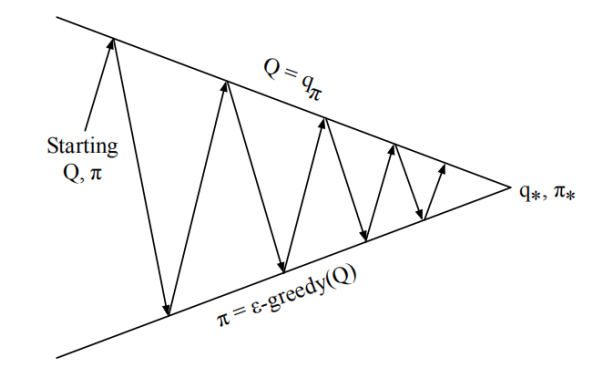
\includegraphics[width=.55\textwidth]{微信图片_20200726205648.png}
    \caption{策略迭代过程示例}
    \label{fig:my_label_1}
\end{figure}
策略迭代通常是一次更新一大步,每次都是求解精准的$V^\pi$。而广义策略迭代,只需要更新一小步,求解的是近似的$V^\pi$,更新多少步,这个随意,并不需要精确的计算$V^\pi$。随着算法的一步步迭代,总可以收敛到最优策略$\pi_\ast$。

我们可以用一个比喻来说明,策略迭代,价值迭代和就地策略迭代之间的关系。策略迭代中,策略估计就相当于全款买房,然后以旧换新;价值迭代,就相当于只付个首付,然后以旧换新;而就地策略迭代基本就是0首付,然后以旧换新。这三个策略最主要的地方就是,对于策略$\pi$价值函数$V^\pi$的计算越来越简单。

\subsection{本章总结}
我们这章介绍的算法都属于动态规划算法,其中对于每一个状态价值函数的估算都依赖于前一时刻各状态价值函数的数值,这种特性我们称之为“bootstrap",都是迭代的算法。这个单词本意是拔靴带,一个比较好的翻译是“自举”,有点自我提升的意思。同时我们注意到,在算法中,我们认为反映环境的所有信息$P(s',r|s,a)$ 是已知的,也就是对马尔可夫决策过程都是全局知道的,即我们已经拥有了对于环境的建模,这种利用反映环境信息的模型来进行计算的特性我们称之为model-based。从某种意义上来说,DP方法本质上还并没有涉及到对于环境的“学习”过程,因为DP没有通过与环境的交互来获取关于环境的信息。设计到对环境的学习,则需要使用以moder-free特性的蒙特卡洛算法的系列算法,将在之后的章节中继续进行描述。

本章主要的思路是介绍如何求解最优策略$\pi^\ast$,主要介绍的是动态规划(DP)算法。其中策略迭代主要的思路可以分成策略评估和策略改进,而由于比较两个策略,需要计算两个价值函数,比较麻烦。所以,介绍了策略改进定理,只需要计算一个策略的价值函数即可。而策略评估需要迭代计算,而策略迭代主体也是一个迭代,涉及到迭代的迭代,算法复杂度非常的高。而之后就提出了价值迭代的方法,价值迭代就是一种特殊的策略迭代,其主要思想是在计算价值函数时,只迭代一步,计算近似的价值函数,这样我们就可以构建价值函数之间的迭代公式,大大的简化了计算。然后价值迭代中针对状态集合中的每一个状态都要更新,需要遍历整个状态空间,大家发现这样更新同样麻烦。于是,科学家们想了一个办法,在第$k$次更新中,不对状态集合$\mathcal{S}$中的每一个状态都更新,而只随机选取其中的某一个状态的$V^k({s_n})$进行更新,其他状态保持不变。这就是就地策略迭代,也是一种特殊的异步策略迭代方法。这三个算法最主要的区别就是,对于策略$\pi$价值函数$V^\pi$的计算越来越简单。整个
思路实际是非常流畅的,从最基础的算法开始,不停的发现问题,改进问题,对算法进行优化。










\end{document}
